% -*- latex -*-
%%%%%%%%%%%%%%%%%%%%%%%%%%%%%%%%%%%%%%%%%%%%%%%%%%%%%%%%%%%%%%%%
%%%%%%%%%%%%%%%%%%%%%%%%%%%%%%%%%%%%%%%%%%%%%%%%%%%%%%%%%%%%%%%%
%%%%
%%%% This text file is part of the lecture slides for
%%%% `Parallel Computing'
%%%% by Victor Eijkhout, copyright 2012-2022
%%%%
%%%% Sessions-slides.tex : about the sessions model
%%%%
%%%%%%%%%%%%%%%%%%%%%%%%%%%%%%%%%%%%%%%%%%%%%%%%%%%%%%%%%%%%%%%%
%%%%%%%%%%%%%%%%%%%%%%%%%%%%%%%%%%%%%%%%%%%%%%%%%%%%%%%%%%%%%%%%

\begin{numberedframe}{Problems with the `world model'}
  MPI is started exactly once:
  \begin{itemize}
  \item MPI can not close down and restart.
  \item Libraries using MPI need to agree on threading and such.
  \end{itemize}
  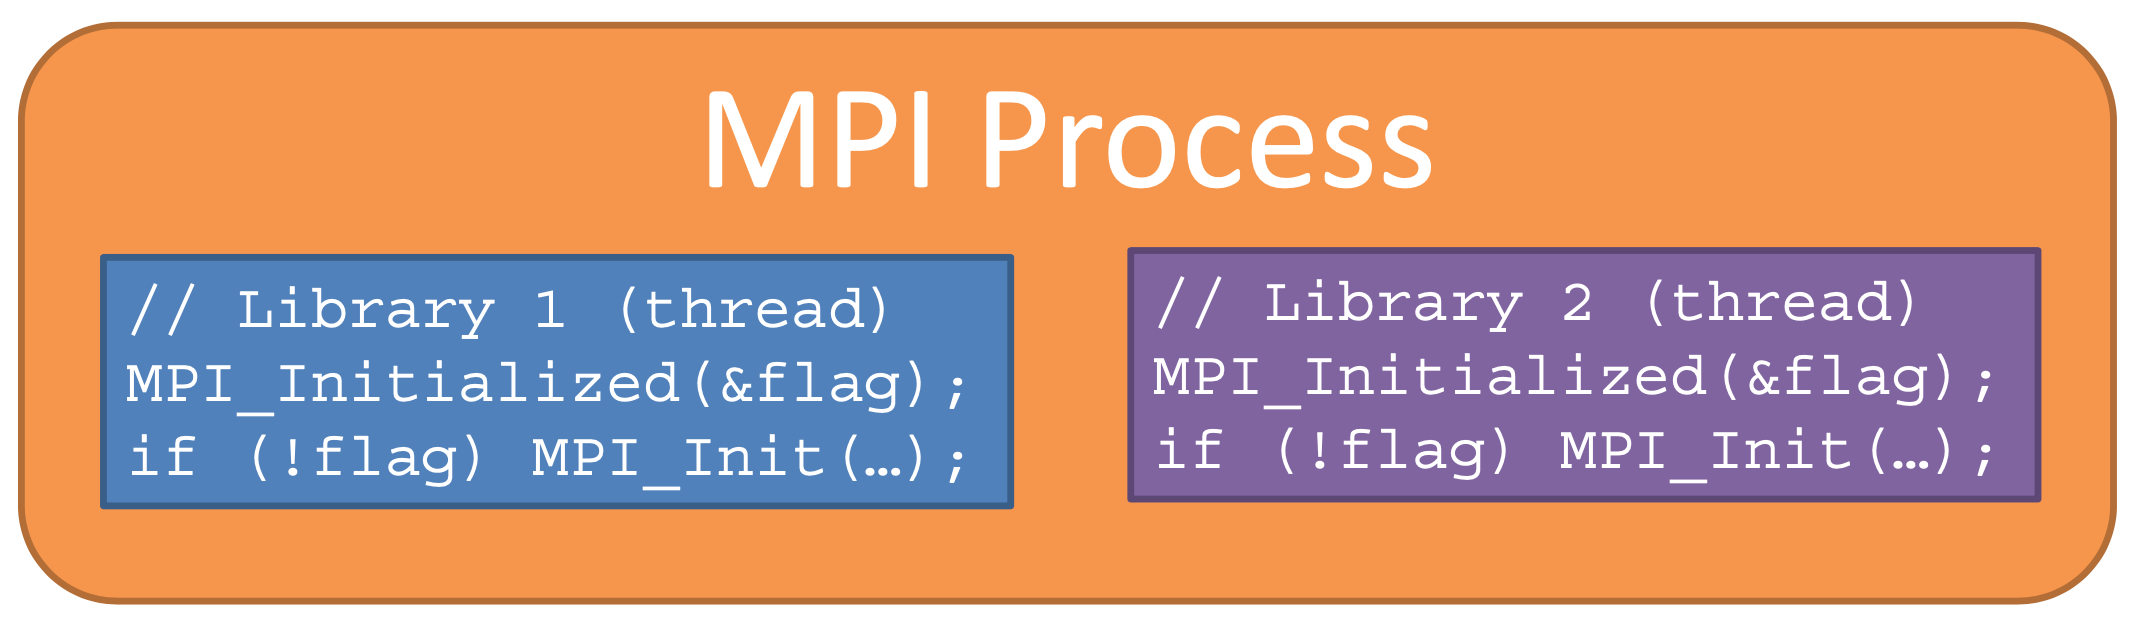
\includegraphics[scale=.2]{mpi_init_conflict}
\end{numberedframe}

\begin{numberedframe}{Sketch of a solution}
  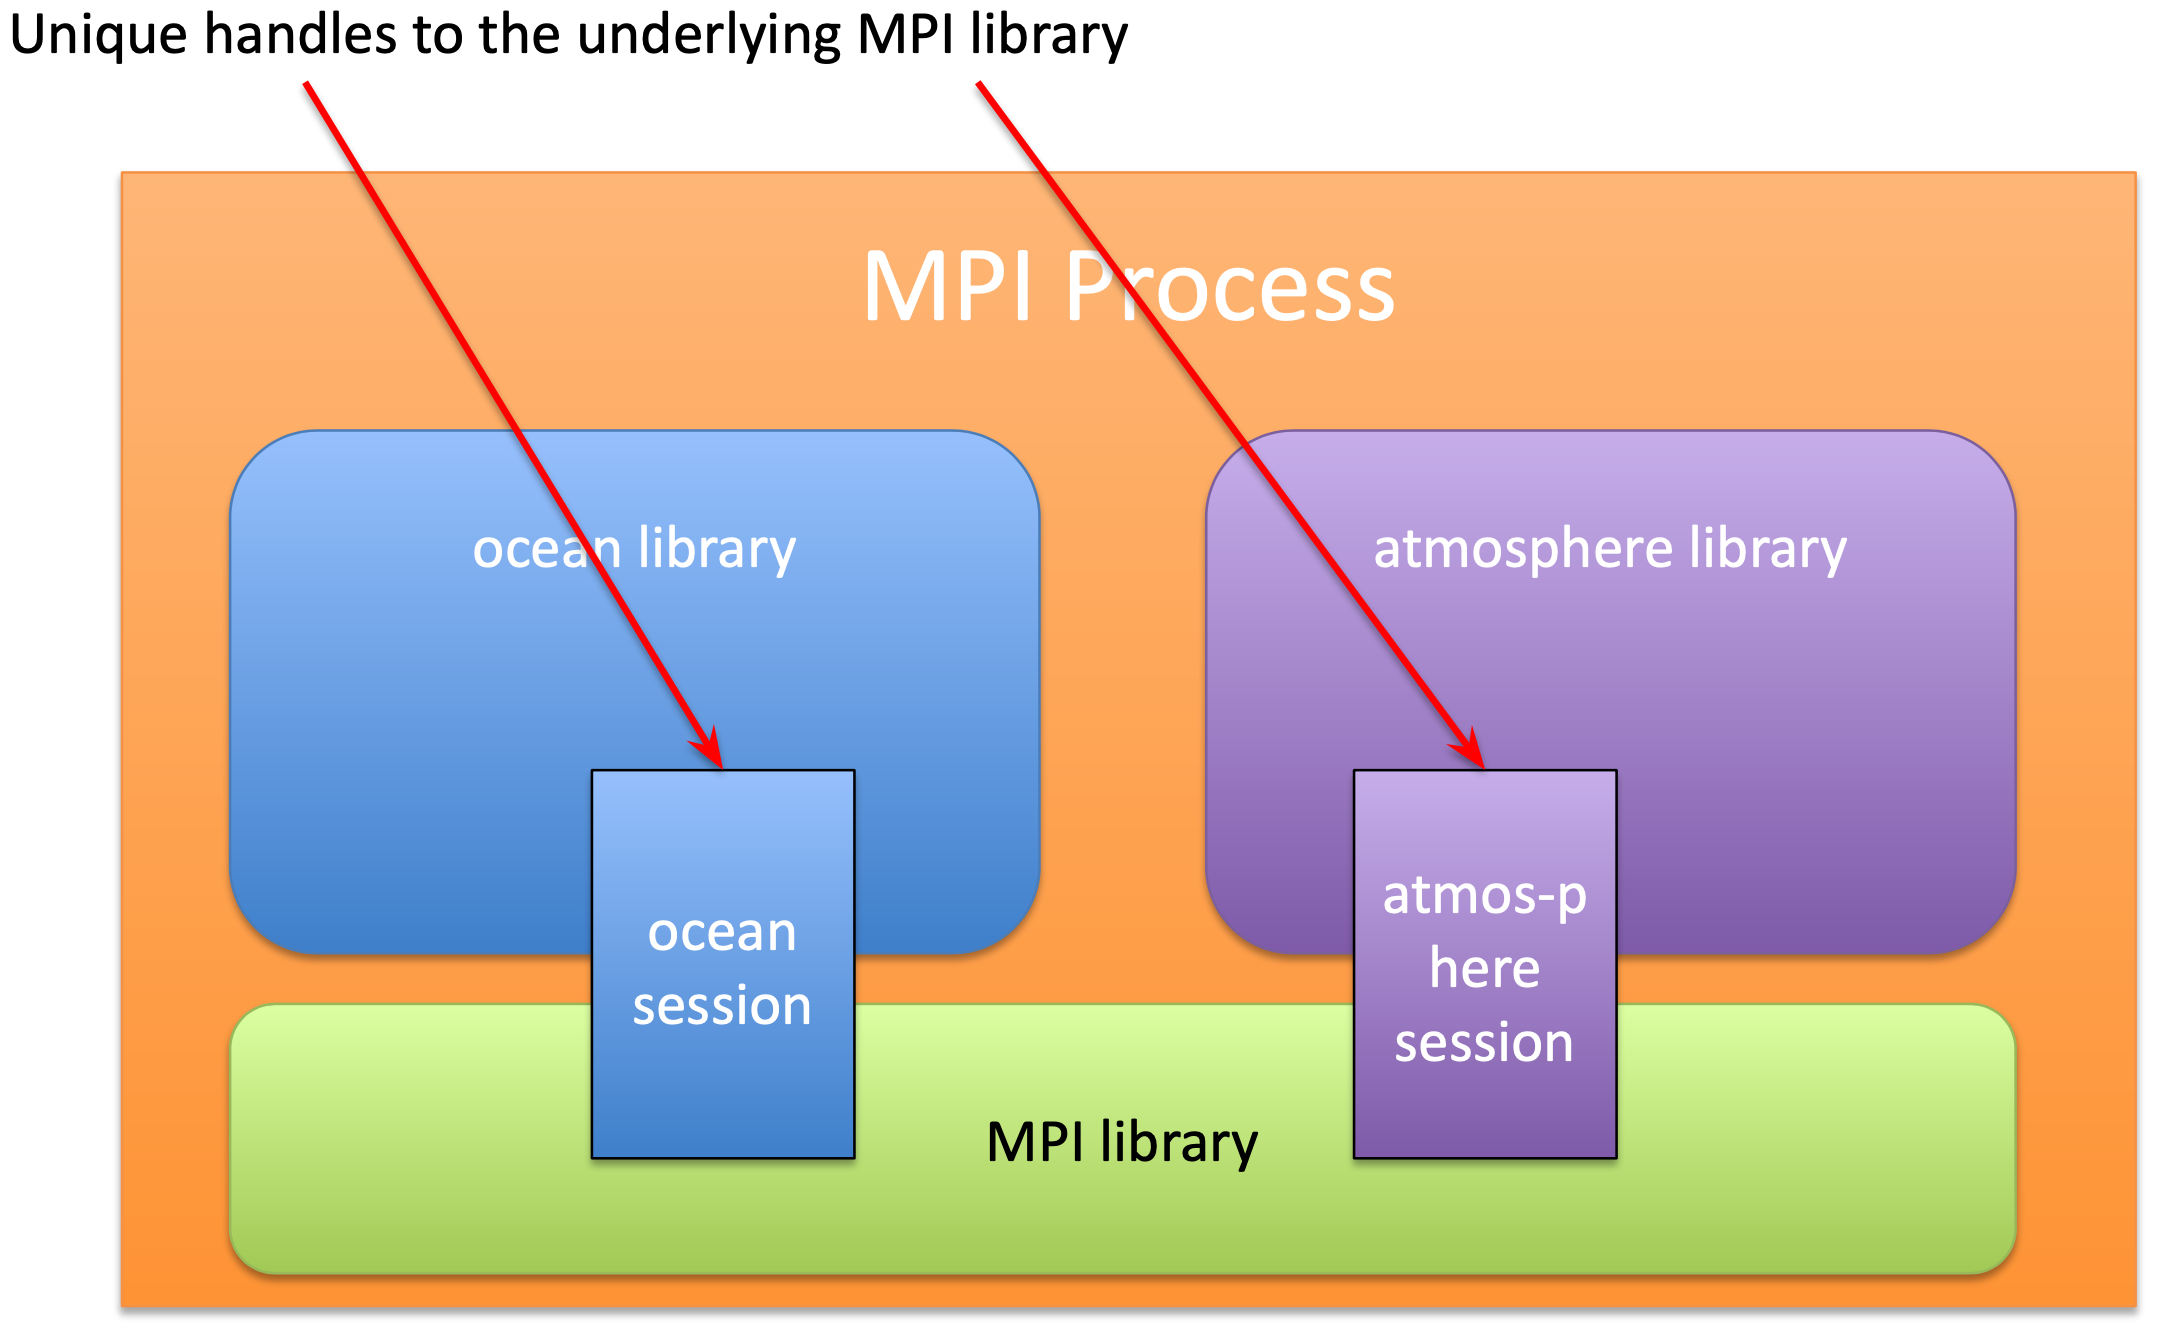
\includegraphics[scale=.2]{mpi_lib_sessions}  
\end{numberedframe}

\begin{numberedframe}{World and session model}
  \begin{itemize}
  \item World model: what you have been doing so far;\\
    Start with \indexmpishow{MPI_COMM_WORLD} and
    make subcommunicators, \\
    or spawn new world communicators and bridge them
  \item Session model: have multiple sessions active,\\
    each starting/ending MPI separately.
  \end{itemize}
\end{numberedframe}

\begin{numberedframe}{Session model}
  \begin{itemize}
  \item Create a session;
  \item a session has multiple `process sets'
  \item from a process set you make a communicator;
  \item Potentially create multiple sessions in one program run
  \item Can not mix objects from multiple simultaneous sessions,\\
    or from session and world model
  \end{itemize}
\end{numberedframe}

\begin{numberedframe}{Session creating}
  \cverbatimsnippet{sessionreq}

  Info object can also be \indexmpishow{MPI_INFO_NULL}, \\
  then
    \cverbatimsnippet{sessioninit}
\end{numberedframe}

\begin{numberedframe}{Session: process sets}
  Process sets, identified by name (not a data type):
  \cverbatimsnippet{sessionpsetq}
  the sets \n{mpi://SELF} and \n{mpi://WORLD} are always defined.
\end{numberedframe}

\begin{numberedframe}{Session: create communicator}
  Process set $\rightarrow$ group $\rightarrow$ communicator
  \cverbatimsnippet{sessioncommworld}
\end{numberedframe}

\begin{numberedframe}{Multiple sessions}
  \cverbatimsnippet{sessionmulti}
\end{numberedframe}

\begin{numberedframe}{Practical use: libraries}
  \cverbatimsnippet{sessionlibdef}
\end{numberedframe}

\begin{numberedframe}{Practical use: main}
  \cverbatimsnippet{sessionlibuse}

  You can not do MPI sends between libraries or library and main\\
  seems reasonable.
\end{numberedframe}
